\section{Critical Context}

A CNN is a class of artificial neural network, or simply neural network, having a basic unit known as a neuron, a mathematical model developed by McCulloch and Pitts (1943), based on biological models of the human brain. Neurons are defined as real numbers, in the form of weighted inputs and a bias, and an activation function, which, given a sum of input values multiplied by weights, plus the bias, generates an output value. The combination of weights and bias represents an encoding, the biological equivalent being a memory. 

Based on the McCulloch-Pitts neuron, Donald Hebb (1949) created the first learning algorithm, that enables a neural network consisting of one single neuron to "learn", or encode, a memory, through an iteration process until, given a cost (or error) function, a set of weights and bias is found such that the same desired output is produced after a number of iterations, and the weights and bias reach stable values while the error is minimized. The Hebbian learning algorithm was able to learn simple tasks such as how to compute the OR truth table, but not more complex tasks such as the XOR truth table. This hindrance is known as a linear separability problem, where, using the inputs as coordinates, the output classes (0,1) of the XOR truth table plotted on a Cartesian plane, cannot be separated by a straight line. Solutions were eventually found, one involving the addition of another layer containing one neuron, known as a "hidden" layer, plus a connection between neurons, plus connections between inputs and the hidden layer neuron. The intuition being, a neural network with more neurons and more connections is able to learn more complex tasks. Such neural network architectures are known as multi-layer perceptrons (MLP) (\cite{Garcez}).  
In the model previously described, inputs are multiplied by weights. In the CNN model, inputs are "convolved" with kernels in the convolutional layers. The concept is borrowed from the digital signal processing domain, where a vector known as a filter or kernel, is combined with a signal to generate a filtered output signal. The operation is expressed by:
\begin{equation}
\label{eqn:1dconv}
conv(s1,s2)[t1]=\sum_{t=0}^{N2-1} s1[t1-t]s2[t]    
\end{equation}
where $s1$ is the input signal, $s2$ is the kernel, $N2$ is the length of $s2$ and $t1$ is the time when input signal $s1$ was acquired. Convolution is similar to cross-correlation (where a measure of similarity between two signals is obtained) except convolution involves "flipping" one of the inputs. This can be observed by the indexing in $s1[t1-t]$ (\cite{Pauwels}). 

For the case of a two-dimensional input and kernel, the operation takes the form:

\begin{equation}
J(x,y) = K * I = \sum_{n,m}K(n,m)I(x-n,y-m) 
\end{equation}
Where $J$ is the convolved signal, $K$ is the kernel, $I$ is the input signal, and $n,m$ are the kernel indexes. We see by the input signal indexing $I(x-n,y-m)$ that both input signal axes are "flipped".

A typical CNN architecture will have a number of convolutional layers, followed by a fully connected MLP, that is, where every unit (neuron) is connected to each other. The convolutional layers are able to compress the input, without losing discriminative information, into a lower dimensional space, where different input categories can be efficiently represented.
The fully-connected MLP layers then perform classification. Convolutional layers in neural networks with the ability to "self-organize", were introduced by the neocognitron network, proposed by \cite{fukushima:neocognitronbc}, particularly efficient for image pattern recognition.

Finding optimal weights and biases for a neural network in a large search space is a mathematically intractable problem that cannot be solved analytically. Eventually it was solved numerically by the use of back-propagation and gradient descent algorithms, like proposed by \cite{Rumelhart:1986we} and \cite{Lecun98gradient-basedlearning}, as well as input normalization and a number of network training optimization algorithms, leading to the wide adoption of neural networks and  "deep" neural networks, with several hidden layers such as CNNs.

The neural network design concepts described, have been implemented in several machine learning libraries such as Facebook's PyTorch, Google's TensorFlow and MATLAB toolkits. TensorFlow has also an embedded port, with a subset functionality. Designing a network from scratch can amount in some cases to writing a few lines of code and networks can be trained on more powerful hardware, and the model then be deployed on less powerful hardware. 

Prior to deep neural networks, computer vision was generally achieved by algorithms dealing with a classification problem, with each pixel in any given image belonging to one of two classes, object and non-object. This is achieved by feature extraction, clustering and segmentation. Feature extraction is the process of engineering features that allow classes to be distinguished. Clustering partitions the feature space into mutually exclusive regions and segmentation assigns each image pixel to one region. The goal being to define regions that can be separated by a hyperplane (with dimension of the feature space minus one) boundary. Colour is generally used as the feature space for images. The practice of "engineering" features, in the age of deep neural networks has become known as "manual" feature extraction, which is time consuming and something we aim to avoid in this proposed work although the practice is by no means outdated.   

Many state-of-the-art machine learning architectures are available as ready-to-use pre-trained models. Implementations of cutting-edge machine learning network architectures are available in public code repositories like GitHub such that one could train the network and create their own model. A model in this context is an actual packaged object that can be used to make predictions given the expected input format and environment.

Together with the network architectures, one very important aspect is the availability of data to train and test neural networks.  The ImageNet (\cite{imagenet_cvpr09}) repository and the related \textit{ImageNet Large Scale Visual Recognition Challenge} spawned a number of 2D image classification deep networks, such as AlexNet, VGGNet, ResNet, etc, that promoted significant advances in 2D computer vision. 

The Fast R-CNN network (\cite{girshick2015fast}) is an example of a deep network designed for image segmentation (Fig.  \ref{fig:fast-r-cnn}). This network is trained end-to-end relying on no engineered features and taking as inputs the image and one optional viewpoint. It consists of convolutional layers followed by a region of interest pooling layer where region proposals are determined, followed by two general fully connected layers followed by one fully connected layer specific to the image, bounding box and viewpoint.

\begin{figure}[ht]
 \centering 
 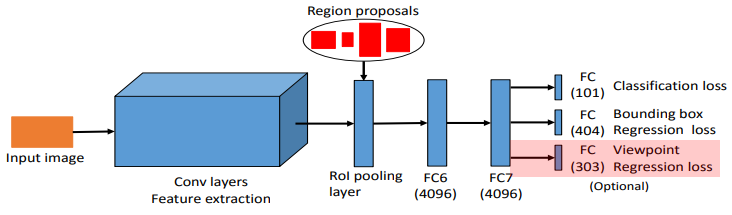
\includegraphics[width=\columnwidth]{figures/Fast-R-CNN-for-object-detection-and-pose-estimation.png}
 \caption{Fast R-CNN architecture. An image and multiple regions of interest (RoIs) are input into a convolutional
network. Each RoI is pooled into a fixed-size feature map and
then mapped to a feature vector by fully connected layers (FCs).
The network has two output vectors per RoI: softmax probabilities
and per-class bounding-box regression offsets. The architecture is
trained end-to-end with a multi-task loss, combining the losses of classification and bounding box regression.}
 \label{fig:fast-r-cnn}
\end{figure}

The 3D computer vision research community, having realised the importance of large publicly available datasets, has created a number of 3D datasets. In the lines of ImageNet, these datasets consist of images labelled, with 3D metadata such as object shape and alignment, usually by crowdsourcing or by setting HITs (Human Intelligence Tasks) in Amazon Mechanical Turk. We discuss these further in section \ref{data-and-tools}.

Large data make computer vision neural networks more robust to overfitting and better at generalising, and in line with increasing the amount of data available for training and testing to improve network performance, one common practice is data augmentation, achieved by blurring, rotating and adding noise to image subsets. Another option is to generate so called synthetic data. Generative adversarial networks (GANs) are a popular choice for creating synthetic data. In the context of 3D objects, this is also possible with open source packages such as OpenSCAD and Blender.  

The ability to generate synthetic training data, for a specific camera intrinsic matrix, with a subset of expected objects in a finite number of poses is attractive, as it constrains the computation and ultimately the size of the model, where the neural network can be designed and trained to solve a very specific problem.

We aim to replicate neural networks such as implemented by  \cite{fan2016point}. The work is seminal in bringing point clouds to the fore of 3D reconstruction, underlining the advantages of the simple and uniform structures that are easier to learn and do not have to encode multiple shape primitives or combinatorial connectivity patterns. The network outputs the point positions in a 3D frame, that is determined by the input image and the inferred viewpoint position (Figure \ref{fig:fan-et-al-vanilla}). 

\begin{figure}[ht]
 \centering 
 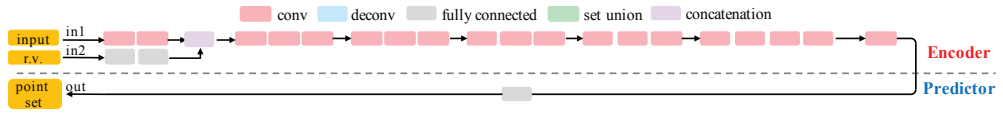
\includegraphics[width=\columnwidth]{figures/fan-et-al-vanilla.png}
 \caption{The PointOutNet \textit{vanilla} architecture}
 \label{fig:fan-et-al-vanilla}
\end{figure}

The network consists of two distinct inputs, the image input and the reference view (r.v.). The image input if followed by two convolutional layers, while the reference view if followed by two fully connected (MLP) layers. Both inputs are combined in a concatenation layer and then followed by a number of convolutional layers. This is the encoding part, where features are extracted. Finally there is a fully connected layer where a prediction (classification) is made to generate an output point set as shown in Figure \ref{fig:fan-et-al-output}. 

\begin{figure}[ht]
 \centering 
 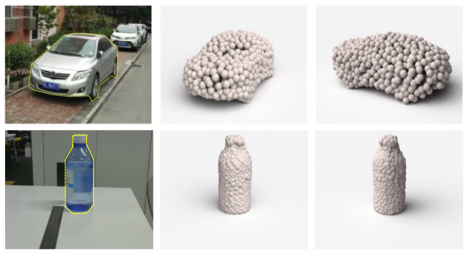
\includegraphics[width=7cm]{figures/fan-et-al-output.png}
 \caption{The PointOutNet 3D point cloud reconstruction from a single image. A segmentation mask is used to indicate the scope of the object in the input images on the left. On the right are the reconstructions viewed at 0 and 90 degrees along azimuth.  Each point is visualised as a small sphere.}
 \label{fig:fan-et-al-output}
\end{figure}

Operations performed by robots which require 3D vision, could benefit from having a compact model, optimised for the camera, generating point clouds that can be used in conjuction with LIDAR point clouds. 

We propose to develop a model prototype, that could be deployed at the embedded, desktop or cloud level. As there are many approaches but as far as we can gather, none specifically aimed at mapping image generated point clouds to be coalesced with LIDAR generated point clouds, the work involves some experimentation, replicating existing models and adapting the workflow to the specific task at hand.




